\documentclass[../PHYS306Notes.tex]{subfiles}

\begin{document}
\subsection{Worksheet - Lagrangian Mechanics with Dissipative Forces \& Constrained Systems}
\begin{p}Write down Newton’sequation of motion for a mass $m$ hanging on a spring with spring constant $k$, equilibrium length $x_0$, and damping coefficient $b$,and subject to a vertical forcing function $F(t)$.
\end{p}
\begin{s}
In one dimension, we have:
\[\sum F = -k(x-x_0) - b\dot{x} - mg + F(t) = m\ddot{x}\]
Where the first term is the spring force, the second term is the air friction, the third term is the gravitational force, and the fourth term is the forcing function. We may rearrange this to say:
\[m\ddot{x} + b\dot{x} + k(x-x_0) = F(t)\]

\end{s}
\begin{p}
In the previous problem, there were nonconservative forces that are not included in our Lagrange formalism. Compare the equation of motion above to the Langrange equation for a mass on a spring without damping and forcing, and suggest how the Lagrange equations should be modified to include friction.
\end{p}
\begin{s}
We consider that Lagrange's equation of motion $\dpd{\LL}{x} = \dod{}{t}\dpd{\LL}{\dot{x}}$ does \textbf{not} account for the nonconservative forces (i.e. the forcing function $F(t)$ and the air friction term $-b\dot{x}$), as the Lagrangian is given by $\LL = T - U = \frac{1}{2}m\dot{x}^2 + mgx + \frac{1}{2}k(x-x_0)^2$ and clearly this does not account for the damping or forcing terms. Without these terms, we have that:
\[\dpd{\LL}{x} = -k(x - x_0) = \dod{}{t}\dpd{\LL}{\dot{x}} = m\ddot{x}\]
But with these terms, we have that:
\[\dpd{\LL}{x} = k(x - x_0) - b\dot{x} + F(t)\]
So the "fix" for nonconservative forces to the Lagrange equations of motion are:
\[\dpd{\LL}{x} + F_{noncons} = \dod{}{t}\dpd{\LL}{\dot{x}}\]
You have to add these in manually because there is no principle of least action for dissipative forces.

\end{s}

\begin{p}
Write down the Lagrangian for the Atwood machine. How many degrees of freedom are there? Pick a generalized coordinate, find the Lagrange equation of motion, and solve it for the acceleration.
\begin{center}
    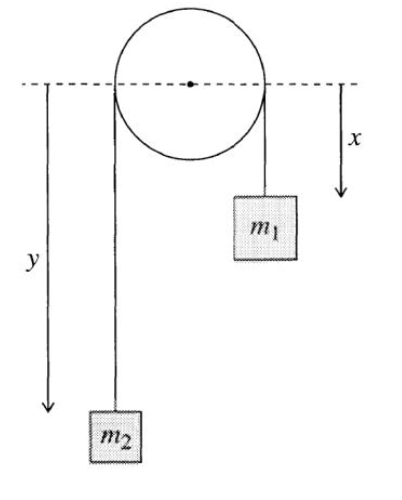
\includegraphics[scale=0.6]{Lecture-4/W4-img1.png}
\end{center}
\end{p}
\begin{s}
There is only one degree of freedom as the motion of one of the masses is completely determined by the other. Let our generalized coordinate be $x$, and we can define the height of the other mass as $y = l - x$ where $l$ is some constant representing the length of the string. The potential energy of the system is given by:
\[U = -m_1gx - m_2g(l-x) = xg(m_2-m_1) - m_2lg\]
The kinetic energy of the system is given by:
\[T = \frac{1}{2}m_1\dot{x}^2 + \frac{1}{2}m_2(-\dot{x})^2 = \frac{1}{2}(m_1 + m_2)\dot{x}^2\]
Hence the Lagrangian of our system is given by:
\[\LL = T - U = \frac{1}{2}(m_1 + m_2)\dot{x}^2 - xg(m_2-m_1) + m_2lg\]
Solving for the equation of motion:
\[\dpd{\LL}{x} = \dod{}{t}\dpd{\LL}{\dot{x}}\]
\[g(m_1 - m_2) = \dod{}{t}(m_1 + m_2)\dot{x}\]
\[g(m_1 - m_2) = (m_1 + m_2)\ddot{x}\]
Hence solving for the acceleration, we get:
\[\ddot{x} = g\frac{m_1 - m_2}{m_1 + m_2}\]
The beauty here is that we really can ignore the constraint forces; if we want to know the motion of the particles, we can use directly the Euler-Lagrange equations of motion. With Newton's laws, we have to keep track of them explicitly; this is why the Lagrangian formulation is often easier.
\end{s}

\begin{p}
A particle of mass $m$ is constrained to move on a frictionless  cylinder of radius $R$, given by the equation $\rho = R$ in cylindrical polar coordinates ($\rho$, $\phi$, $z$). Besides the force of constraint (the normal force of the cylinder), the only force on the mass is a force $F = -kr$ directed toward the origin. Using $z$ and $\phi$ as generalized coordinates, find the Lagrangian $\LL$ Write down and solve Lagrange's equations and describe the motion. 
\end{p}
\begin{s}
The "spring" potential energy from the force directed towards the origin is given by $U_{spr} = \frac{1}{2}k(R^2 + z^2)$. The kinetic energy of the particle is given as $T = \frac{1}{2}m\dot{\v{r}}^2 = \frac{1}{2}m(\dot{z}^2 + R^2\dot{\phi}^2)$. The Lagrangian is therefore given by:
\[\LL = T - U = \frac{1}{2}m(\dot{z}^2 + R^2\dot{\phi}^2) - \frac{1}{2}k(R^2 + z^2)\]
Now we use the EL equations to find the equations of motion for $z$ and $phi$. Starting with $z$:
\[\dpd{\LL}{z} = \dod{}{t}\dpd{\LL}{\dot{z}}\]
\[- kz = m\ddot{z}\]
The solution to this differential equation is simple harmonic motion with frequency $\omega = \sqrt{\frac{k}{m}}$:
\[z(t) = A\cos(\omega t) + B\sin(\omega t)\]
Next for $\phi$:
\[\dpd{\LL}{\phi} = \dod{}{t}\dpd{\LL}{\dot{\phi}}\]
\[0 = \dod{}{t}\left(mR^2\dot{\phi}\right)\]
\[0 = mR^2\ddot{\phi}\]
Hence (as we knew already from angular momentum conservation) we find that $\ddot{\phi}$ is conserved and hence $\dot{\phi}$ is constant. 
\end{s}

\end{document}